\documentclass[12pt]{article}
\usepackage{titling}
\usepackage{graphicx}
\usepackage{caption}
\usepackage{subcaption}

\newcommand{\subtitle}[1]{%
  \posttitle{%
    \par\end{center}
    \begin{center}\large#1\end{center}
    \vskip0.5em}%
}

				

\begin{document}

%

\title{Measures of Cognitive Distance}			% used by \maketitle
\author{Johannes  Castner, }		% used by \maketitle
\date \today	
\maketitle

\section{Some Basic Axioms for a Distance Function}

\begin{equation}
d(i, j)\geq 0
\end{equation}

\begin{equation}
d(i, i)= 0
\end{equation}

\begin{equation}
d(i, j)=d(j, i)
\end{equation}

It would be great if the distance function were to satisfy ultrametric inequality, i.e.

\begin{equation}
d(i, j)\leq max \lbrace d(i, l), d(j, l) \rbrace.
\end{equation}

The reason why this last property is desirable is that (as Weitzman sketched a proof in his paper) the following would be guaranteed to hold for the Weitzman diversity measure, $V$, for all relevant objects $j$:

\begin{equation}
V(Q \cup j)-V(Q) = d(j, Q)
\end{equation}

where $Q$ is any subset of the set of objects, $S$, over which the diversity is to be measured and $d(j, Q)=min_{i\in Q} d(j, i)$.  Moreover, only if the distance measure is ultrametric does (5) hold for all relevant objects.     

\subsection{Playing around with distances for single arcs}

$$(1/2)*d(+, -) = d(+, \emptyset)= d(-, \emptyset) = d(0, \emptyset) \geq$$

This distance can be thought of as one where the probability of the positive and the negative relation is equal and thus it can be expressed as the string: $(++++0000----)$ for $(1/2)*d(+, -1)$. This is the string for which the Shannon Entropy is maximized and equal to $1.58496$. 

$$d(+, \ominus)=d(m, 0)=d(m, \emptyset) \geq $$

For $d(+, \ominus)$ the probability of the relation being zero is a bit higher than for $d(+, -1)$ and thus the string representation is $(++++00000---)$, where there is an additional $0$ and one less $-$. The Shannon Entropy is less and equal to $1.55459$.

$$d(\ominus, \oplus) \geq d(m, \oplus)=d(m, \ominus) \geq$$

For $d(\ominus, \oplus)$, for example, the probability of the relationship being positive/negative is reduced and the probability of it being zero is increased and thus the string representation is $+++000000---$, for which the Shannon Entropy is $1.5$. 

$$d(+, 0)=d(-, 0) \geq$$

For $d(+, 0)$ The probability of the relationship being $0$ is further increased and the probability that it is positive is as before and thus the string representation is $++++000000--$, for which the Shannon Entropy is $1.45915$. 

$$d(+, u)=d(-,u)=d(0, u) \geq$$

For $d(+, u)$ the probability of a positive relation is even further increased and the probability of the relation being zero or negative is equal but low. Thus the string representation is $++++++++00--$ for which the Shannon Entropy is $1.25163$. 

$$d(+, m)= d(-, m) \geq d(m , u) \geq$$

For $d(+, m)$ the probability of the relationship being zero is $0$ but the probability of it being negative is still there and thus the string representation is $++++++++----$ for which the Shannon entropy is $0.9183$.

$$d(-, \ominus)=d(+, \oplus)=d(0, \ominus)=d(0, \oplus)$$

For $d(+, \oplus)$ the probability that the relationship is zero is small but positive and the probability that it is positive is quite high and thus the string representation is $++++++++++00$ for which the Shannon Entropy is $0.65002$. 

\subsection{A Distance Function for Cognitive Maps}

The function $d(i, j)$ I propose to measure the distance between two cognitive maps $(i,j)$ is based on two dimensions of these maps: their content and their structure. Content distance refers to the difference in the information content of two maps and it is measured as the sum of the difference in information entropy when each map is augmented with the other. The event of interest in the computation of this information entropy is any message $m$ containing an assertion of the type "X increases (decreases, or has 0 effect on, ) Y". The information entropy of person A's graph when put in relation to the dyad (A,B) is calculated as follows:

$$\sum_{Graph(A)} m*p(m) * log 2p(m),$$

where 

$$p(m^*)= \frac{\#m^*}{\sum m, \forall m \in Graph(A) \bigcup Graph(B)}.$$ 
 
Here, $\#m^*$ denotes the number of times message $m^*$ appears in both graphs and it takes values in $(1, 2)$ (either one politician has asserted the existence of causal arc $m^*$ and the other one has not, or both have).

This measure of content distance has two desirable properties: it increases with the number of causal links that are in the union, but not in the intersection of the two graphs, relative to the size of the intersection, and it also increases in the difference in the number of causal arcs contained in each graph. \\
Whereas content distance is concerned with the difference in ``what'' politicians say, structural distance focuses on the difference in ``how'' they think and argue, as illustrated in Figures ~\ref{graphs1} and ~\ref{graphs2} . For example, a directed labeled graph may have many negative loops, indicating belief in equilibria, whereas positive loops represent beliefs in runaway feedbacks.      

\begin{figure}
        \centering
        \begin{subfigure}[A]{0.7\textwidth}
                \centering
                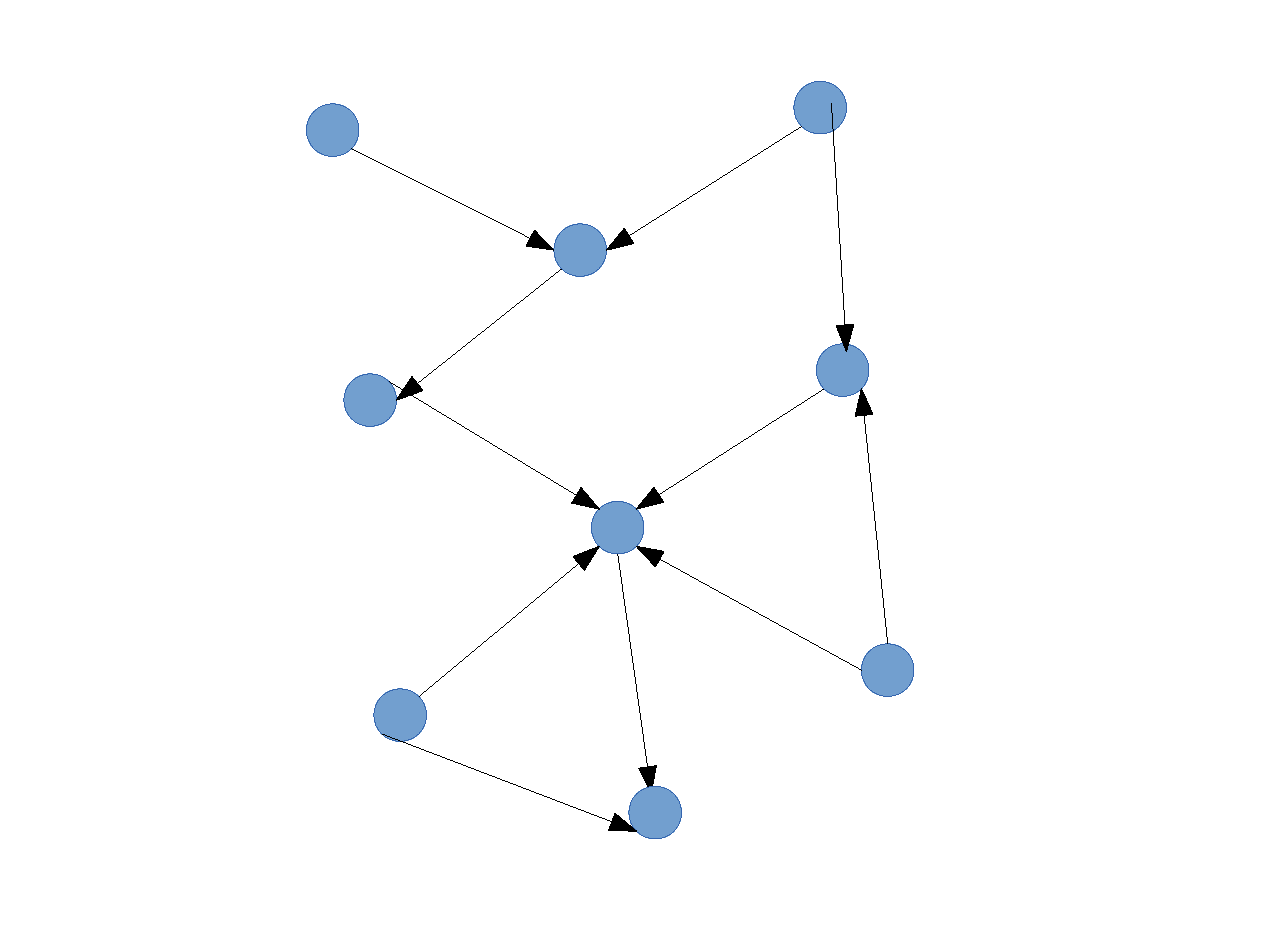
\includegraphics[width=\textwidth]{GraphA.pdf}
                \subcaption{}
                \label{grapha}
        \end{subfigure}%
        ~ %add desired spacing between images, e. g. ~, \quad, \qquad etc.
          %(or a blank line to force the subfigure onto a new line)
        \begin{subfigure}[B]{0.7\textwidth}
                \centering
                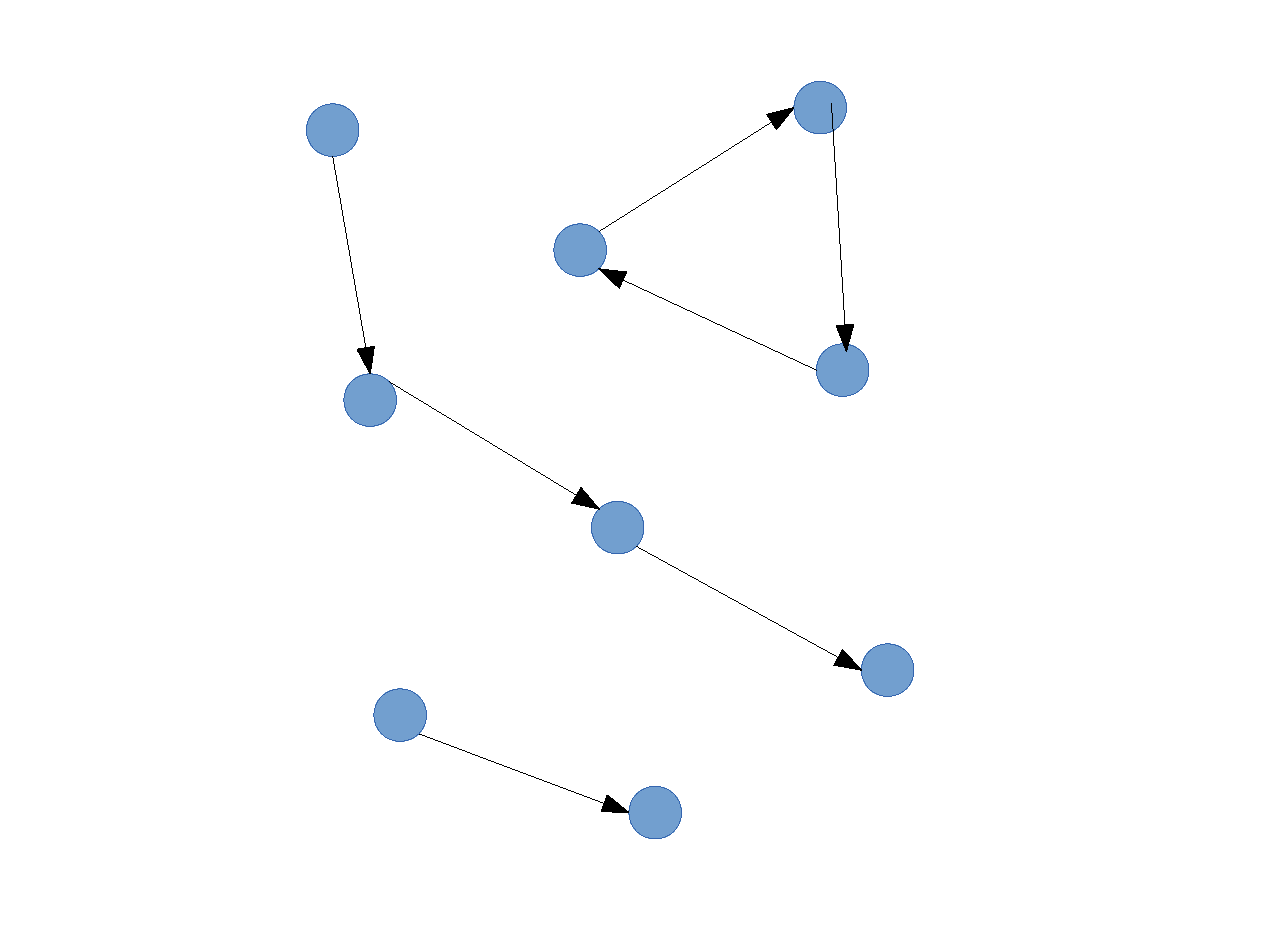
\includegraphics[width=\textwidth]{GraphB.pdf}
                \subcaption{}
                \label{graphb}
        \end{subfigure}
        ~ %add desired spacing between images, e. g. ~, \quad, \qquad etc.
          %(or a blank line to force the subfigure onto a new line)
        \caption{Two structurally very different Cognitive Maps. a) is very connected and has no cycles, for example, while b) is much more fragmented, has one cycle and otherwise chains causes and effects linearly. While graph a) might look very close to the graphs in Figure ~\ref{graphs2}, note that a) has not a single cycle, while both graphs in Figure ~\ref{graphs2} have many cycles.}\label{graphs1}
\end{figure}

There are other important structural aspects that I consider, such as the difference in how connected two graphs are, as connection indicates how fragmented the belief system is. To compute structural distance, I obtain the empirical distributions over structural properties and compare them using a statistical distance measure (the Vasershtein metric; Vasershtein, 1969). 

\begin{figure}
        \centering
        \begin{subfigure}[C]{0.7\textwidth}
                \centering
                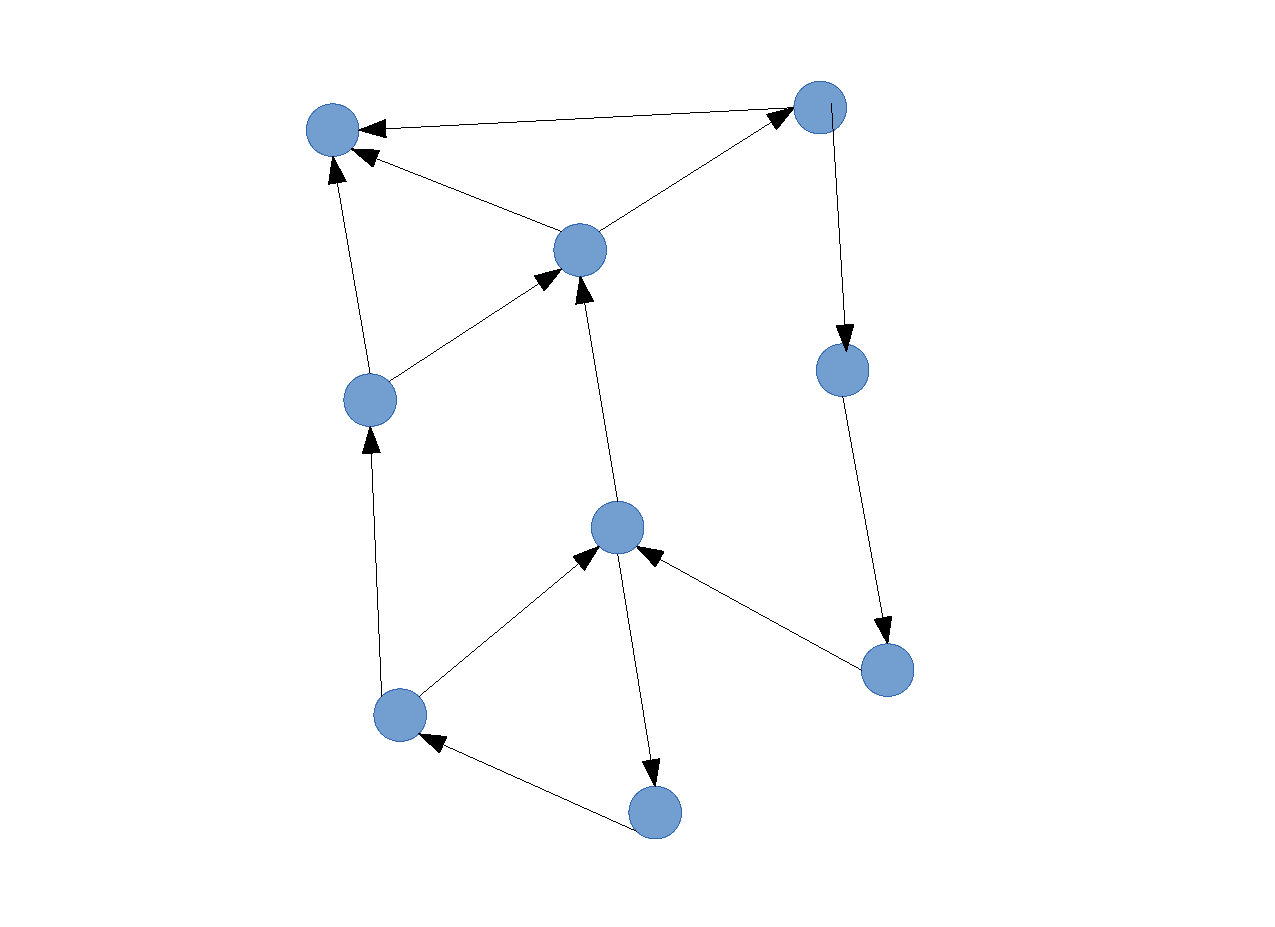
\includegraphics[width=\textwidth]{GraphC.pdf}
                \subcaption{}
                \label{graphc}
        \end{subfigure}%
        ~ %add desired spacing between images, e. g. ~, \quad, \qquad etc.
          %(or a blank line to force the subfigure onto a new line)
        \begin{subfigure}[D]{0.7\textwidth}
                \centering
                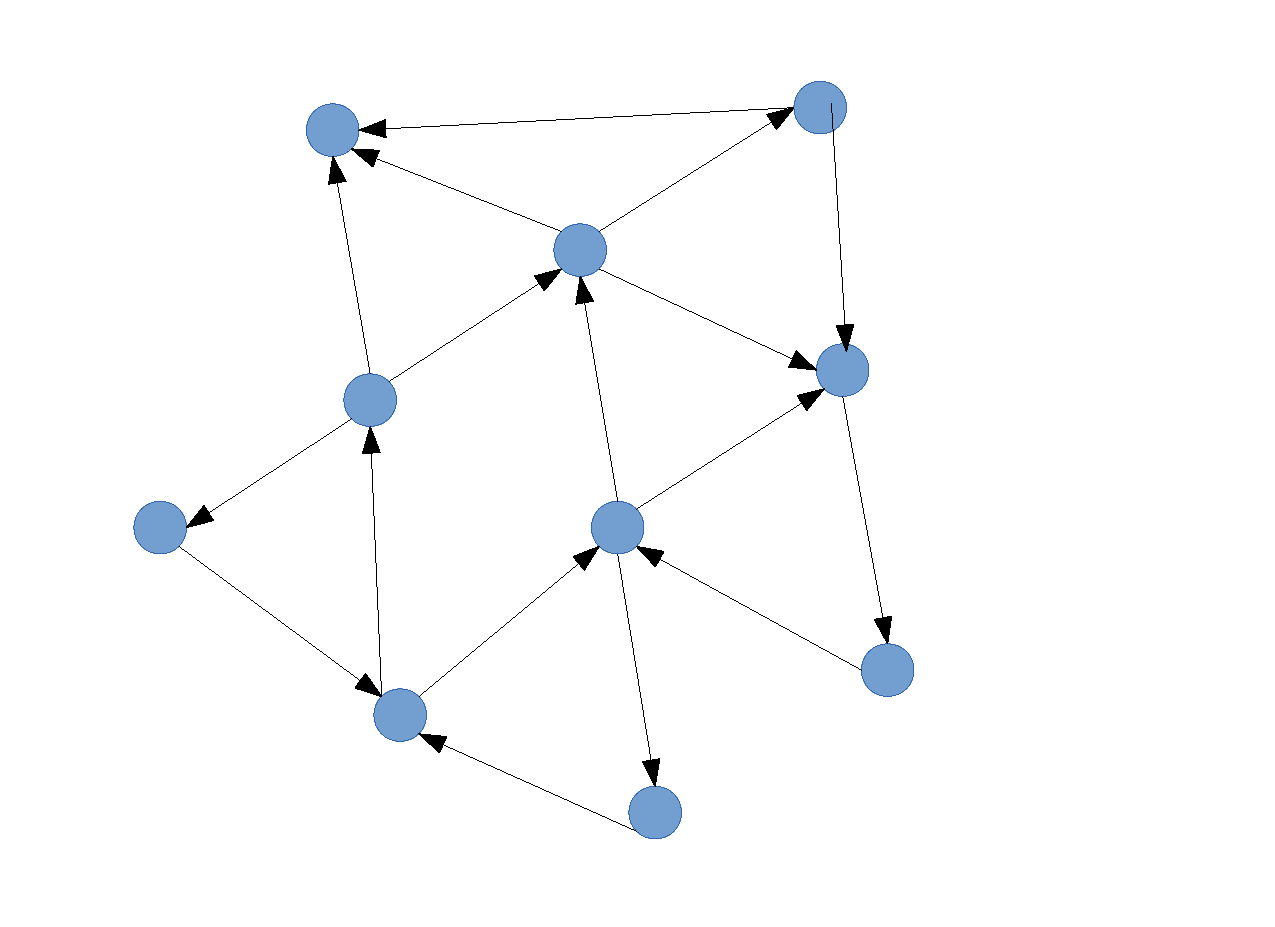
\includegraphics[width=\textwidth]{GraphD.pdf}
                \subcaption{}
                \label{graphd}
        \end{subfigure}
        ~ %add desired spacing between images, e. g. ~, \quad, \qquad etc.
          %(or a blank line to force the subfigure onto a new line)
        \caption{Two structurally very similar Cognitive Maps. Both graphs have many cycles (their owners believe in many feedbacks) and they are quite connected. The labels on either the edges or the nodes in these figures have been omitted to visually highlight the structural aspects of distance between these graphs.}\label{graphs2}
\end{figure}

\section{Axioms of the Weitzman Measures of Diversity}

The proofs for the following axioms can be found in Weitzman 1992. 
\begin{itemize}
\item Monotonicity in types. 

This property is simply that diversity weakly increases if one type is added. 

\item Link Property

For all $S$, $|S|\geq 2$, there exists at least one type $j \in S$, such that

$$V(S)= d(j, S \setminus j) + V(S\setminus j)$$ 

In the case that $d(\cdot, \cdot)$ is ultrametric, the Link Property holds for all $j$ and $S$. 

\item Twin Property

Suppose there is a $k \not\in S$ and some $j \in S$ such that 
$d(j, k)=0$ and $d(k, i)=d(j, i)$, $\forall i \in S$, 

$$\Longrightarrow V(S\cup k)=V(S).$$ 

\item Continuity in Distances

Let $|S|=|S^{'}|$. Let $\phi(\cdot)$ be a one to one function, mapping $S$ onto $S^{'}$.

Then $\forall \epsilon > 0$ there exist a $\delta > 0$ such that $\sum\sum|d(i, j)-d(\phi(i), \phi(j))|<\delta$ implies that:

$$|V(S)-V(S^{'})|<\epsilon$$

\item Monotonicity in Distances

Let $|S|=|S^{'}|\geq 2$. Let $\phi(\cdot)$ be a one to one function, mapping $S$ onto $S^{'}$.

Suppose that
$$d(\phi(i), \phi(j)) \geq d(i, j), \forall i, j \in S, i\not=j.$$

Then
$$V(S^{'}) \geq V(S).$$

\item Maximum Diversity that can be added by a single Type

If type $k \not\in S$ is added to the collection $S$, then

$$V(S\cup k) \leq V(S) + D(k, S),$$

where $D(k, S)=max_{i \in S} d(k, i).$



\end{itemize}
\end{document}             % End of document.
